\documentclass[british]{emisa}

\usepackage{blindtext}
\usepackage{booktabs}

\begin{document}
\lstset{language=TeX}
\begin{article}{%
% Enter your bibliography database file here. Make sure to use UTF-8 character encoding!
\bibliography{emisa.bib}
\title[Insert shorttitle for headlines here]{Enter full title here}
\subtitle{Enter subtitle here, or leave empty}
\author*{FirstName LastName}{email@address.org}
\address{Enter affiliation of first and corresponding author here.  Note that only the starred version of author* accepts a second argument providing an email address for the corresponding author.}
\author{FirstName LastName}
\address{Enter affiliation of second author here. Add further authors following the source code scheme.}

\abstract{Enter abstract here} 
\keywords{Enter at a minimum three keywords here. Keyword1 \and Keyword2 \and Keyword3}
\acknowledgements{Enter acknowledgements here.}
\authornote{If your submission is based on a prior publication and revises / extends the prior work, enter a note on all prior publications with full citation.}
%, \eg this article extends an earlier conference publication published in the conference proceedings, see \cite{}.}
}


\section{Introduction}
\label{intro}
Enter your text here \parencite{Mittelbach.2004}. Remember to use \texttt{biber} instead of \texttt{bibtex} for processing the bibliography (.bib) file(s). \textcite{Mittelbach.2004} provide an introduction to \LaTeX{} which should be complemented by more recent readings (\ie certain parts of \cite{Mittelbach.2004} are probably outdated). Note the differences when using \verb|\parencite{}| or \verb|\textcite{}| or \verb|\cite{}| in the examples above. See Sec.~\ref{sec:bib} for advice on how to enter bibliographic data in the .bib file.


\section{Floating objects ('floats')}\label{sec:1}
Enter your text here. 

\subsection{Subsection title}\label{sec:2}
Provide a unique label for each section, table, figure, listing and algorithm for referencing purposes (see, \eg, Sec.~\ref{sec:3} and Tab.~\ref{enter-a-unique-label-here}). 




\subsection{Figures}\label{sec:3}
\begin{figure}[htbp]
\centering
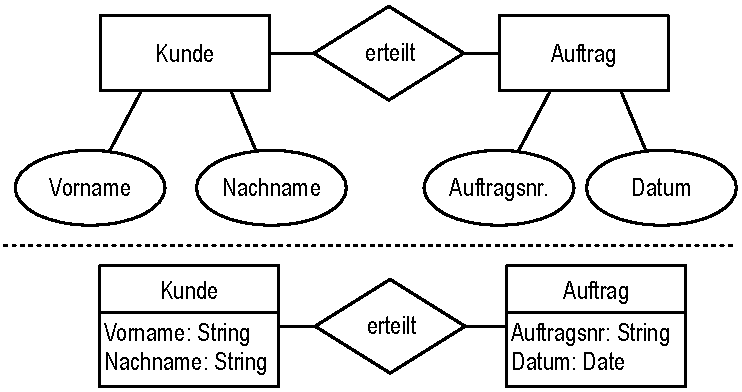
\includegraphics[width=\columnwidth]{figure.pdf}
\caption{Enter your single-column figure caption here.}
\label{default}
\end{figure}

\begin{figure*}[htb]
\centering
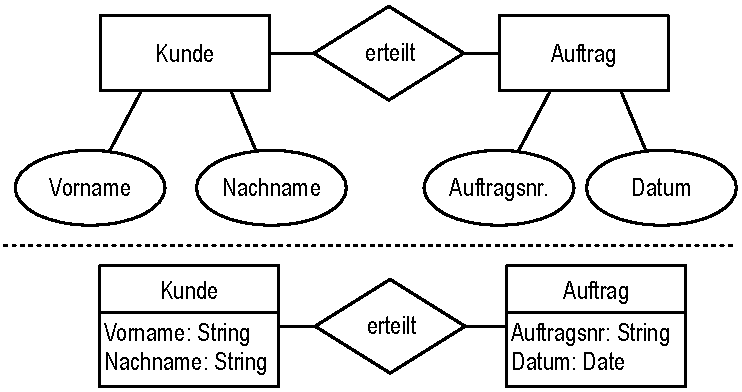
\includegraphics[width=\textwidth]{figure.pdf}
\caption{Enter your double-column figure caption here.}
\label{default}
\end{figure*}

\blindtext



\subsection{Tables}\label{sec:tables}
Typeset tables as floats in double-columns using \verb|\begin{table*}|, see Tab.~\ref{tab:unique-label} for an example.

\begin{table*}[tb]
\centering
\caption{Enter your table caption above the table here.}
\begin{tabular}{llllll}
\toprule
column head1 & column head2 & column head3 & column head4 & column head5 & column head6\\
\midrule
cell1 & cell2 & cell3 & cell4 & cell5 & cell6\\
cell1 & cell2 & cell3 & cell4 & cell5 & cell6\\
cell1 & cell2 & cell3 & cell4 & cell5 & cell6\\
cell1 & cell2 & cell3 & cell4 & cell5 & cell6\\
cell1 & cell2 & cell3 & cell4 & cell5 & cell6\\
\bottomrule
\end{tabular}
\label{tab:unique-label}
\end{table*}

%\blindtext[2]\ Lorem ipsum hoc nunc.\footnote{Use footnotes only when absolutely necessary.}


%\blindtext[1]



\section{Formatting the bibliography}\label{sec:bib}

Please make sure to properly enter all data for each entry in the bibliographic database (.bib). Pay special attention to formatting names and page numbers, see Listing~\ref{lst:1} for an example (\cite{key1}) formatted properly in the references section (use \verb|--| between page numbers and \verb|{}| around multiple word surnames!). 

\begin{lstlisting}[float,caption={Enter your single-column listing caption here.},label={lst:1}]
@ARTICLE{key1,
  author = {{van der Aalst}, W. M. P. 
  and {van Hee}, K. M. 
  and {van Werf}, J. M. 
  and Verdonk, M.},
  title = {{Auditing 2.0: Using 
  Process Mining to Support 
  Tomorrow's Auditor}},
  journal = {Computer},
  year = {2010},
  volume = {43},
  pages = {90--93},
  number = {3}
}
\end{lstlisting}



\section{Source code listings}\label{sec:listings}

For typesetting source code listings, use the \verb|sourcecode|, \verb|java| or \verb|pseudocode| environments provided by the document class. All three environments are customized from the lstlistings package. 

See Listing~\ref{lst:2} for an example of a double-column listing.

\begin{lstlisting}[float=*htbp,caption={Enter your double-column listing caption here. Note that the listing width is too wide. Correct by entering a newline before, \eg, 'Tomorrow'.},label={lst:2}]
@ARTICLE{key1,
  author = {{van der Aalst}, W. M. P. and {van Hee}, K. M. and 
  {van Werf}, J. M. and Verdonk, M.},
  title = {{Auditing 2.0: Using Process Mining to Support Tomorrow's Auditor}},
  journal = {Computer},
  year = {2010},
  volume = {43},
  pages = {90--93},
  number = {3}
}
\end{lstlisting}

%\blindtext[3]


\section{Formatting pseudocode}\label{sec:algorithm}
XXX Nutzung von algorithm-Umgebung illustrieren XXX 



%\begin{table}[htbp]
%\caption{Enter your table caption here.}
%\begin{tabular*}{\linewidth}{lll}
%\toprule
%column head1 & column head2 & column head3\\
%\midrule
%cell1 & cell2 & cell3\\
%cell1 & cell2 & cell3\\
%\bottomrule
%\end{tabular*}
%\label{enter-a-unique-label-here}
%\end{table}
%

%\begin{table}[htbp]
%\caption{Enter your table caption here.}
%\begin{tabular}{lll}
%\toprule
%column head1 & column head2 & column head3\\
%\midrule
%cell1 & cell2 & cell3\\
%cell1 & cell2 & cell3\\
%\bottomrule
%\end{tabular}
%\label{enter-a-unique-label-here}
%\end{table}

%
%
%\section{Introduction and installation}
%
%This reference guide provides a detailed description of the \LaTeX2e\ EMISA document class version 2.x (newer than 2015-11-17) plus auxiliary files and their features designed to facilitate the preparation of submissions to EMISA.
%
%The EMISA \LaTeX\ package consists of the EMISA \LaTeX\ class \texttt{emisa.cls}, the BibLaTeX bibliography style \texttt{emisa.bbx} and the BibLaTeX control file \texttt{emisa.bbx}. The package is (soon) available from the Comprehensive \TeX\ Archive Network (CTAN, \url{https://ctan.org}).
%
%
%The package also includes the present instructions and guidelines for authors on formatting the \LaTeX\ source file of the manuscript to achieve a pleasing and typographically consistent visual appearance of the published document (\eg with respect to figures and tables).
%
%Follow these instructions and guidelines to set up your files, to type in your text, typeset figures, tables and listings, and to obtain a consistent typesetting in accordance with the journal's style specifications. 
%It is recommended to use these instructions as a checklist before submitting your manuscript to the journal's online submission system at \url{https://emisa-journal.org}.
%
%Note that the instructions are not intended as a general introduction to \LaTeX2e{} or \TeX{} (see \url{https://www.ctan.org/tex-archive/info/lshort/english/} for the free \enquote{The not so Short Introduction to LaTeX}). 
%
%%• The Reference Guide describing SVMono features with regards to their functionality.
%%Tip: Use it as a reference if you need to alter or enhance the default settings of the SVMono document class and/or the templates.
%
%%The documentation in the Springer SVMono tool package is not intended to be a general introduction to LATEX2ε or TEX. For this we refer you to [1–3].
%%Should we refer in this tool package to standard tools or packages that are not installed on your system, please consult the Comprehensive TEX Archive Network (CTAN) at [4–6].
%
%
%
%\section{Installation}
%
%The EMISA package should be installable via regular package installers (\eg the \TeX{}Live Utility). For a manual installation, install the three files in the same subfolder as your manuscript source file.  XXX
%
%
%
%\section{Preliminaries}
%
%%Preparing a manuscript for submission to \enquote{Enterprise Modelling and Information Systems Architectures -- An International Journal} (EMISA) must make use of the EMISA \LaTeX\ class provided by the journal. 
%
%The manuscript processing at EMISA is entirely based on UTF-8 (Unicode) file encodings. All source code files including the \LaTeX\ source files (.tex) and the bibliography file (.bib) \emph{must} be submitted in UTF-8 file encoding (\ie Unicode). The editorial office \emph{will not} process any other file encoding and, thus, will have to reject your manuscript if its source files are not encoded in UTF-8. Make sure that all files submitted to the journal are properly encoded in UTF-8.
%
%EMISA uses the following tool chain and sequence to produce the final proof of your manuscript: \texttt{pdflatex}, \texttt{biber}, \texttt{pdflatex}, \texttt{pdflatex}. Please note that the newer BibLaTeX package is used for typesetting the citations and references (\ie bibliography section) in combination with the \texttt{biber} tool rather than the outdated \texttt{bibtex} tool.
%% with a corresponding bibtex style (for a documentation of the BibLaTeX package, see XXX).  
%
%
%
%
%\section{Shortcuts to common acronyms and abbreviations}
%
%The EMISA class provides shortcuts to the following acronyms and abbreviations which should be used instead of typographically problematic alternatives, \ie, use \verb|\eg| (or \verb|\eg{}|) instead of typing \texttt{e.g.}\ in the source code. The use of the following shortcuts is \emph{strongly} recommended:
%
%\begin{tabular}{ll}
% \verb|\eg| & \eg{}\\
% \verb|\ie| & \ie{}\\
% \verb|\cf| & \cf{}\\
%\ldots
%\end{tabular}
%

\printbibliography
\end{article}
\end{document}
\endinput

